% Options for packages loaded elsewhere
\PassOptionsToPackage{unicode}{hyperref}
\PassOptionsToPackage{hyphens}{url}
\PassOptionsToPackage{dvipsnames,svgnames,x11names}{xcolor}
%
\documentclass[
  letterpaper,
  DIV=11,
  numbers=noendperiod]{scrartcl}

\usepackage{amsmath,amssymb}
\usepackage{lmodern}
\usepackage{iftex}
\ifPDFTeX
  \usepackage[T1]{fontenc}
  \usepackage[utf8]{inputenc}
  \usepackage{textcomp} % provide euro and other symbols
\else % if luatex or xetex
  \usepackage{unicode-math}
  \defaultfontfeatures{Scale=MatchLowercase}
  \defaultfontfeatures[\rmfamily]{Ligatures=TeX,Scale=1}
\fi
% Use upquote if available, for straight quotes in verbatim environments
\IfFileExists{upquote.sty}{\usepackage{upquote}}{}
\IfFileExists{microtype.sty}{% use microtype if available
  \usepackage[]{microtype}
  \UseMicrotypeSet[protrusion]{basicmath} % disable protrusion for tt fonts
}{}
\makeatletter
\@ifundefined{KOMAClassName}{% if non-KOMA class
  \IfFileExists{parskip.sty}{%
    \usepackage{parskip}
  }{% else
    \setlength{\parindent}{0pt}
    \setlength{\parskip}{6pt plus 2pt minus 1pt}}
}{% if KOMA class
  \KOMAoptions{parskip=half}}
\makeatother
\usepackage{xcolor}
\setlength{\emergencystretch}{3em} % prevent overfull lines
\setcounter{secnumdepth}{-\maxdimen} % remove section numbering
% Make \paragraph and \subparagraph free-standing
\ifx\paragraph\undefined\else
  \let\oldparagraph\paragraph
  \renewcommand{\paragraph}[1]{\oldparagraph{#1}\mbox{}}
\fi
\ifx\subparagraph\undefined\else
  \let\oldsubparagraph\subparagraph
  \renewcommand{\subparagraph}[1]{\oldsubparagraph{#1}\mbox{}}
\fi

\usepackage{color}
\usepackage{fancyvrb}
\newcommand{\VerbBar}{|}
\newcommand{\VERB}{\Verb[commandchars=\\\{\}]}
\DefineVerbatimEnvironment{Highlighting}{Verbatim}{commandchars=\\\{\}}
% Add ',fontsize=\small' for more characters per line
\usepackage{framed}
\definecolor{shadecolor}{RGB}{241,243,245}
\newenvironment{Shaded}{\begin{snugshade}}{\end{snugshade}}
\newcommand{\AlertTok}[1]{\textcolor[rgb]{0.68,0.00,0.00}{#1}}
\newcommand{\AnnotationTok}[1]{\textcolor[rgb]{0.37,0.37,0.37}{#1}}
\newcommand{\AttributeTok}[1]{\textcolor[rgb]{0.40,0.45,0.13}{#1}}
\newcommand{\BaseNTok}[1]{\textcolor[rgb]{0.68,0.00,0.00}{#1}}
\newcommand{\BuiltInTok}[1]{\textcolor[rgb]{0.00,0.23,0.31}{#1}}
\newcommand{\CharTok}[1]{\textcolor[rgb]{0.13,0.47,0.30}{#1}}
\newcommand{\CommentTok}[1]{\textcolor[rgb]{0.37,0.37,0.37}{#1}}
\newcommand{\CommentVarTok}[1]{\textcolor[rgb]{0.37,0.37,0.37}{\textit{#1}}}
\newcommand{\ConstantTok}[1]{\textcolor[rgb]{0.56,0.35,0.01}{#1}}
\newcommand{\ControlFlowTok}[1]{\textcolor[rgb]{0.00,0.23,0.31}{#1}}
\newcommand{\DataTypeTok}[1]{\textcolor[rgb]{0.68,0.00,0.00}{#1}}
\newcommand{\DecValTok}[1]{\textcolor[rgb]{0.68,0.00,0.00}{#1}}
\newcommand{\DocumentationTok}[1]{\textcolor[rgb]{0.37,0.37,0.37}{\textit{#1}}}
\newcommand{\ErrorTok}[1]{\textcolor[rgb]{0.68,0.00,0.00}{#1}}
\newcommand{\ExtensionTok}[1]{\textcolor[rgb]{0.00,0.23,0.31}{#1}}
\newcommand{\FloatTok}[1]{\textcolor[rgb]{0.68,0.00,0.00}{#1}}
\newcommand{\FunctionTok}[1]{\textcolor[rgb]{0.28,0.35,0.67}{#1}}
\newcommand{\ImportTok}[1]{\textcolor[rgb]{0.00,0.46,0.62}{#1}}
\newcommand{\InformationTok}[1]{\textcolor[rgb]{0.37,0.37,0.37}{#1}}
\newcommand{\KeywordTok}[1]{\textcolor[rgb]{0.00,0.23,0.31}{#1}}
\newcommand{\NormalTok}[1]{\textcolor[rgb]{0.00,0.23,0.31}{#1}}
\newcommand{\OperatorTok}[1]{\textcolor[rgb]{0.37,0.37,0.37}{#1}}
\newcommand{\OtherTok}[1]{\textcolor[rgb]{0.00,0.23,0.31}{#1}}
\newcommand{\PreprocessorTok}[1]{\textcolor[rgb]{0.68,0.00,0.00}{#1}}
\newcommand{\RegionMarkerTok}[1]{\textcolor[rgb]{0.00,0.23,0.31}{#1}}
\newcommand{\SpecialCharTok}[1]{\textcolor[rgb]{0.37,0.37,0.37}{#1}}
\newcommand{\SpecialStringTok}[1]{\textcolor[rgb]{0.13,0.47,0.30}{#1}}
\newcommand{\StringTok}[1]{\textcolor[rgb]{0.13,0.47,0.30}{#1}}
\newcommand{\VariableTok}[1]{\textcolor[rgb]{0.07,0.07,0.07}{#1}}
\newcommand{\VerbatimStringTok}[1]{\textcolor[rgb]{0.13,0.47,0.30}{#1}}
\newcommand{\WarningTok}[1]{\textcolor[rgb]{0.37,0.37,0.37}{\textit{#1}}}

\providecommand{\tightlist}{%
  \setlength{\itemsep}{0pt}\setlength{\parskip}{0pt}}\usepackage{longtable,booktabs,array}
\usepackage{calc} % for calculating minipage widths
% Correct order of tables after \paragraph or \subparagraph
\usepackage{etoolbox}
\makeatletter
\patchcmd\longtable{\par}{\if@noskipsec\mbox{}\fi\par}{}{}
\makeatother
% Allow footnotes in longtable head/foot
\IfFileExists{footnotehyper.sty}{\usepackage{footnotehyper}}{\usepackage{footnote}}
\makesavenoteenv{longtable}
\usepackage{graphicx}
\makeatletter
\def\maxwidth{\ifdim\Gin@nat@width>\linewidth\linewidth\else\Gin@nat@width\fi}
\def\maxheight{\ifdim\Gin@nat@height>\textheight\textheight\else\Gin@nat@height\fi}
\makeatother
% Scale images if necessary, so that they will not overflow the page
% margins by default, and it is still possible to overwrite the defaults
% using explicit options in \includegraphics[width, height, ...]{}
\setkeys{Gin}{width=\maxwidth,height=\maxheight,keepaspectratio}
% Set default figure placement to htbp
\makeatletter
\def\fps@figure{htbp}
\makeatother

\usepackage{fvextra}
\usepackage{svg}
\DefineVerbatimEnvironment{Highlighting}{Verbatim}{breaklines,commandchars=\\\{\}}
\KOMAoption{captions}{tableheading}
\makeatletter
\makeatother
\makeatletter
\makeatother
\makeatletter
\@ifpackageloaded{caption}{}{\usepackage{caption}}
\AtBeginDocument{%
\ifdefined\contentsname
  \renewcommand*\contentsname{Table of contents}
\else
  \newcommand\contentsname{Table of contents}
\fi
\ifdefined\listfigurename
  \renewcommand*\listfigurename{List of Figures}
\else
  \newcommand\listfigurename{List of Figures}
\fi
\ifdefined\listtablename
  \renewcommand*\listtablename{List of Tables}
\else
  \newcommand\listtablename{List of Tables}
\fi
\ifdefined\figurename
  \renewcommand*\figurename{Figure}
\else
  \newcommand\figurename{Figure}
\fi
\ifdefined\tablename
  \renewcommand*\tablename{Table}
\else
  \newcommand\tablename{Table}
\fi
}
\@ifpackageloaded{float}{}{\usepackage{float}}
\floatstyle{ruled}
\@ifundefined{c@chapter}{\newfloat{codelisting}{h}{lop}}{\newfloat{codelisting}{h}{lop}[chapter]}
\floatname{codelisting}{Listing}
\newcommand*\listoflistings{\listof{codelisting}{List of Listings}}
\makeatother
\makeatletter
\@ifpackageloaded{caption}{}{\usepackage{caption}}
\@ifpackageloaded{subcaption}{}{\usepackage{subcaption}}
\makeatother
\makeatletter
\@ifpackageloaded{tcolorbox}{}{\usepackage[many]{tcolorbox}}
\makeatother
\makeatletter
\@ifundefined{shadecolor}{\definecolor{shadecolor}{rgb}{.97, .97, .97}}
\makeatother
\makeatletter
\makeatother
\ifLuaTeX
  \usepackage{selnolig}  % disable illegal ligatures
\fi
\IfFileExists{bookmark.sty}{\usepackage{bookmark}}{\usepackage{hyperref}}
\IfFileExists{xurl.sty}{\usepackage{xurl}}{} % add URL line breaks if available
\urlstyle{same} % disable monospaced font for URLs
\hypersetup{
  colorlinks=true,
  linkcolor={blue},
  filecolor={Maroon},
  citecolor={Blue},
  urlcolor={Blue},
  pdfcreator={LaTeX via pandoc}}

\author{}
\date{}

\begin{document}
\begin{titlepage}

    \newcommand{\HRule}{\rule{\linewidth}{0.5mm}}
    
    \center
    
    \textsc{\LARGE GSMST }\\[0.3cm]
    \textsc{\Large Applications of Linear Algebra }\\[0.3cm]
    \textsc{\Large in Programming}\\[0.5cm]
    
    \HRule \\[0.4cm]
    { \huge \bfseries Error Correcting Lab}\\[0.03cm]
    \HRule \\[1.5cm]
    
    \begin{minipage}{0.4\textwidth}
    \begin{flushleft} \large
    \emph{Submitted By:}\\
    Anish Goyal \\4th Period
    \end{flushleft}
    \end{minipage}
    ~
    \begin{minipage}{0.4\textwidth}
    \begin{flushright} \large
    \emph{Submitted To:} \\
    Mrs. Denise Stiffler\\Educator
    \end{flushright}
    \end{minipage}\\[1cm]
    
    {\large May 8, 2023}\\[1cm]
    
    
\includegraphics{logo.png}\\[1cm]
    \vfill
    \end{titlepage}
\newpage

\ifdefined\Shaded\renewenvironment{Shaded}{\begin{tcolorbox}[borderline west={3pt}{0pt}{shadecolor}, frame hidden, interior hidden, boxrule=0pt, enhanced, breakable, sharp corners]}{\end{tcolorbox}}\fi

\renewcommand*\contentsname{Table of contents}
{
\hypersetup{linkcolor=}
\setcounter{tocdepth}{4}
\tableofcontents
}
\newpage{}

\hypertarget{review-questions}{%
\subsection{Review Questions}\label{review-questions}}

\hypertarget{what-does-the-notation-f-a-longrightarrow-b-mean}{%
\subsubsection{\texorpdfstring{What does the notation
\(f : A \longrightarrow B\)
mean?}{What does the notation f : A \textbackslash longrightarrow B mean?}}\label{what-does-the-notation-f-a-longrightarrow-b-mean}}

\(f\) is a function whose domain is the set \(A\) and codomain is the
set \(B\). AKA: \(f\) is a function that maps \(A\) to \(B\).

\hypertarget{what-are-the-criteria-for-f-to-be-an-invertible-function}{%
\subsubsection{\texorpdfstring{What are the criteria for \(f\) to be an
invertible
function?}{What are the criteria for f to be an invertible function?}}\label{what-are-the-criteria-for-f-to-be-an-invertible-function}}

\begin{itemize}
\tightlist
\item
  \(f \circ g\) is defined and the identity function on the domain of
  \(g\)
\item
  \(g \circ f\) is defined and the identity function on the domain of
  \(f\)
\end{itemize}

\hypertarget{what-is-the-associativity-of-functional-composition}{%
\subsubsection{What is the associativity of functional
composition?}\label{what-is-the-associativity-of-functional-composition}}

\(h \circ (g \circ f) = (h \circ g) \circ f\)

\hypertarget{what-are-the-criteria-for-a-function-to-be-a-probability-function}{%
\subsubsection{What are the criteria for a function to be a probability
function?}\label{what-are-the-criteria-for-a-function-to-be-a-probability-function}}

\begin{itemize}
\tightlist
\item
  The function must output a non-negative real number for all inputs.
\item
  The function must be measurable, meaning it must correspond to some
  set that can be assigned a probability.
\end{itemize}

\hypertarget{what-is-the-fundamental-principle-of-probability-theory}{%
\subsubsection{What is the Fundamental Principle of Probability
Theory?}\label{what-is-the-fundamental-principle-of-probability-theory}}

The probability of an event is the sum of probabilities.

\hypertarget{if-the-input-to-an-invertible-function-is-chosen-randomly-according-to-the-uniform-distribution-what-is-the-distribution-of-the-output}{%
\subsubsection{If the input to an invertible function is chosen randomly
according to the uniform distribution, what is the distribution of the
output?}\label{if-the-input-to-an-invertible-function-is-chosen-randomly-according-to-the-uniform-distribution-what-is-the-distribution-of-the-output}}

The output will also have a uniform distribution. This is because an
invertible function is a one-to-one mapping, so it preserves the
uniformity of the distribution. In other words, every possible output
value will have the same probability of being produced, as every
possible input value has the same probability of being chosen.

\hypertarget{problems}{%
\subsection{0.8 Problems}\label{problems}}

\hypertarget{problem-0.8.1}{%
\subsubsection{Problem 0.8.1}\label{problem-0.8.1}}

increments(L)\\
input: list L of numbers\\
output: list of numbers in which the ith element is one plus the ith
element Example: increments({[}1, 5, 7{]}) should return {[}2, 6, 8{]}

\begin{Shaded}
\begin{Highlighting}[numbers=left,,]
\KeywordTok{def}\NormalTok{ increments(L): }\ControlFlowTok{return}\NormalTok{ [x}\OperatorTok{+}\DecValTok{1} \ControlFlowTok{for}\NormalTok{ x }\KeywordTok{in}\NormalTok{ L]}
\BuiltInTok{print}\NormalTok{(increments([}\DecValTok{1}\NormalTok{, }\DecValTok{5}\NormalTok{, }\DecValTok{7}\NormalTok{]))}
\end{Highlighting}
\end{Shaded}

\begin{verbatim}
[2, 6, 8]
\end{verbatim}

\hypertarget{problem-0.8.2}{%
\subsubsection{Problem 0.8.2}\label{problem-0.8.2}}

cubes(L)\\
input: list L of numbers\\
output: list of numbers in which the ith element is the cube of the ith
element of L.\\
Example: given {[}1, 2, 3{]} return {[}1, 8, 27{]}

\begin{Shaded}
\begin{Highlighting}[numbers=left,,]
\KeywordTok{def}\NormalTok{ cubes(L): }\ControlFlowTok{return}\NormalTok{[x}\OperatorTok{**}\DecValTok{3} \ControlFlowTok{for}\NormalTok{ x }\KeywordTok{in}\NormalTok{ L]}
\BuiltInTok{print}\NormalTok{(cubes([}\DecValTok{1}\NormalTok{, }\DecValTok{2}\NormalTok{, }\DecValTok{3}\NormalTok{]))}
\end{Highlighting}
\end{Shaded}

\begin{verbatim}
[1, 8, 27]
\end{verbatim}

\hypertarget{problem-0.8.3}{%
\subsubsection{Problem 0.8.3}\label{problem-0.8.3}}

tuple\_sum(A, B)\\
input: lists A and B of the same length, where each element in each list
is a pair (x, y) of numbers\\
output: list of pairs (x, y) in which the first element of the ith pair
is the sum of the first element of the ith pair in A and the first
element of the ith pair in B\\
Example: given lists {[}(1, 2), (10, 20){]} and {[}(3, 4), (30, 40){]},
return {[}(4, 6), (40, 60){]}

\begin{Shaded}
\begin{Highlighting}[numbers=left,,]
\KeywordTok{def}\NormalTok{ tuple\_sum(A, B): }\ControlFlowTok{return}\NormalTok{ [(x[}\DecValTok{0}\NormalTok{]}\OperatorTok{+}\NormalTok{y[}\DecValTok{0}\NormalTok{], x[}\DecValTok{1}\NormalTok{]}\OperatorTok{+}\NormalTok{y[}\DecValTok{1}\NormalTok{]) }\ControlFlowTok{for}\NormalTok{ x, y }\KeywordTok{in} \BuiltInTok{zip}\NormalTok{(A, B)]}
\NormalTok{A}\OperatorTok{=}\NormalTok{ [(}\DecValTok{1}\NormalTok{, }\DecValTok{2}\NormalTok{), (}\DecValTok{10}\NormalTok{, }\DecValTok{20}\NormalTok{)]}
\NormalTok{B }\OperatorTok{=}\NormalTok{ [(}\DecValTok{3}\NormalTok{, }\DecValTok{4}\NormalTok{), (}\DecValTok{30}\NormalTok{, }\DecValTok{40}\NormalTok{)]}
\BuiltInTok{print}\NormalTok{(tuple\_sum(A, B))}
\end{Highlighting}
\end{Shaded}

\begin{verbatim}
[(4, 6), (40, 60)]
\end{verbatim}

\hypertarget{problem-0.8.4}{%
\subsubsection{Problem 0.8.4}\label{problem-0.8.4}}

inv\_dict(d)\\
input: dictionary d representing an invertible function f\\
output: dictionary representing the inverse of f, the returned
dictionary's keys are the value of d and its values are the keys of d\\
Example: given an English-French dictionary:\\
\{`thank you' : `merci', `goodbye' : `au revoir'\}\\
return a French-English dictionary:\\
\{`merci' : `thank you', `au revoir' : `goodbye'\}

\begin{Shaded}
\begin{Highlighting}[numbers=left,,]
\KeywordTok{def}\NormalTok{ inv\_dict(d): }\ControlFlowTok{return}\NormalTok{ \{v: k }\ControlFlowTok{for}\NormalTok{ k, v }\KeywordTok{in}\NormalTok{ d.items()\}}
\NormalTok{d }\OperatorTok{=}\NormalTok{ \{}\StringTok{\textquotesingle{}thank you\textquotesingle{}}\NormalTok{ : }\StringTok{\textquotesingle{}merci\textquotesingle{}}\NormalTok{, }\StringTok{\textquotesingle{}goodbye\textquotesingle{}}\NormalTok{ : }\StringTok{\textquotesingle{}au revoir\textquotesingle{}}\NormalTok{\}}
\BuiltInTok{print}\NormalTok{(inv\_dict(d))}
\end{Highlighting}
\end{Shaded}

\begin{verbatim}
{'merci': 'thank you', 'au revoir': 'goodbye'}
\end{verbatim}

\hypertarget{problem-0.8.5}{%
\subsubsection{Problem 0.8.5}\label{problem-0.8.5}}

First write a procedure row with the following spec:\\
input: integer p, integer n\\
output: n-element list such that element i is p+i\\
Example: given p = 10 and n = 4, return {[}10, 11, 12, 13{]}\\
Next, write a comprehension whose value is a 15-element list of
20-element lists such that the jth element of the ith list is i+j. You
can use row(p, n) in your comprehension.\\
Finally, write the same comprehension but without using row(p, n). Hint:
replace the call to row(p, n) with the comprehension that forms the body
of row (p, n)\\

\begin{Shaded}
\begin{Highlighting}[numbers=left,,]
\KeywordTok{def}\NormalTok{ row(p, n): }\ControlFlowTok{return}\NormalTok{ [p}\OperatorTok{+}\NormalTok{i }\ControlFlowTok{for}\NormalTok{ i }\KeywordTok{in} \BuiltInTok{range}\NormalTok{(n)]}
\BuiltInTok{print}\NormalTok{(row(}\DecValTok{10}\NormalTok{, }\DecValTok{4}\NormalTok{))}
\BuiltInTok{print}\NormalTok{([row(i, }\DecValTok{20}\NormalTok{) }\ControlFlowTok{for}\NormalTok{ i }\KeywordTok{in} \BuiltInTok{range}\NormalTok{(}\DecValTok{15}\NormalTok{)])}
\BuiltInTok{print}\NormalTok{([[i}\OperatorTok{+}\NormalTok{j }\ControlFlowTok{for}\NormalTok{ j }\KeywordTok{in} \BuiltInTok{range}\NormalTok{(}\DecValTok{20}\NormalTok{)] }\ControlFlowTok{for}\NormalTok{ i }\KeywordTok{in} \BuiltInTok{range}\NormalTok{(}\DecValTok{15}\NormalTok{)])}
\end{Highlighting}
\end{Shaded}

\begin{verbatim}
[10, 11, 12, 13]
[[0, 1, 2, 3, 4, 5, 6, 7, 8, 9, 10, 11, 12, 13, 14, 15, 16, 17, 18, 19], [1, 2, 3, 4, 5, 6, 7, 8, 9, 10, 11, 12, 13, 14, 15, 16, 17, 18, 19, 20], [2, 3, 4, 5, 6, 7, 8, 9, 10, 11, 12, 13, 14, 15, 16, 17, 18, 19, 20, 21], [3, 4, 5, 6, 7, 8, 9, 10, 11, 12, 13, 14, 15, 16, 17, 18, 19, 20, 21, 22], [4, 5, 6, 7, 8, 9, 10, 11, 12, 13, 14, 15, 16, 17, 18, 19, 20, 21, 22, 23], [5, 6, 7, 8, 9, 10, 11, 12, 13, 14, 15, 16, 17, 18, 19, 20, 21, 22, 23, 24], [6, 7, 8, 9, 10, 11, 12, 13, 14, 15, 16, 17, 18, 19, 20, 21, 22, 23, 24, 25], [7, 8, 9, 10, 11, 12, 13, 14, 15, 16, 17, 18, 19, 20, 21, 22, 23, 24, 25, 26], [8, 9, 10, 11, 12, 13, 14, 15, 16, 17, 18, 19, 20, 21, 22, 23, 24, 25, 26, 27], [9, 10, 11, 12, 13, 14, 15, 16, 17, 18, 19, 20, 21, 22, 23, 24, 25, 26, 27, 28], [10, 11, 12, 13, 14, 15, 16, 17, 18, 19, 20, 21, 22, 23, 24, 25, 26, 27, 28, 29], [11, 12, 13, 14, 15, 16, 17, 18, 19, 20, 21, 22, 23, 24, 25, 26, 27, 28, 29, 30], [12, 13, 14, 15, 16, 17, 18, 19, 20, 21, 22, 23, 24, 25, 26, 27, 28, 29, 30, 31], [13, 14, 15, 16, 17, 18, 19, 20, 21, 22, 23, 24, 25, 26, 27, 28, 29, 30, 31, 32], [14, 15, 16, 17, 18, 19, 20, 21, 22, 23, 24, 25, 26, 27, 28, 29, 30, 31, 32, 33]]
[[0, 1, 2, 3, 4, 5, 6, 7, 8, 9, 10, 11, 12, 13, 14, 15, 16, 17, 18, 19], [1, 2, 3, 4, 5, 6, 7, 8, 9, 10, 11, 12, 13, 14, 15, 16, 17, 18, 19, 20], [2, 3, 4, 5, 6, 7, 8, 9, 10, 11, 12, 13, 14, 15, 16, 17, 18, 19, 20, 21], [3, 4, 5, 6, 7, 8, 9, 10, 11, 12, 13, 14, 15, 16, 17, 18, 19, 20, 21, 22], [4, 5, 6, 7, 8, 9, 10, 11, 12, 13, 14, 15, 16, 17, 18, 19, 20, 21, 22, 23], [5, 6, 7, 8, 9, 10, 11, 12, 13, 14, 15, 16, 17, 18, 19, 20, 21, 22, 23, 24], [6, 7, 8, 9, 10, 11, 12, 13, 14, 15, 16, 17, 18, 19, 20, 21, 22, 23, 24, 25], [7, 8, 9, 10, 11, 12, 13, 14, 15, 16, 17, 18, 19, 20, 21, 22, 23, 24, 25, 26], [8, 9, 10, 11, 12, 13, 14, 15, 16, 17, 18, 19, 20, 21, 22, 23, 24, 25, 26, 27], [9, 10, 11, 12, 13, 14, 15, 16, 17, 18, 19, 20, 21, 22, 23, 24, 25, 26, 27, 28], [10, 11, 12, 13, 14, 15, 16, 17, 18, 19, 20, 21, 22, 23, 24, 25, 26, 27, 28, 29], [11, 12, 13, 14, 15, 16, 17, 18, 19, 20, 21, 22, 23, 24, 25, 26, 27, 28, 29, 30], [12, 13, 14, 15, 16, 17, 18, 19, 20, 21, 22, 23, 24, 25, 26, 27, 28, 29, 30, 31], [13, 14, 15, 16, 17, 18, 19, 20, 21, 22, 23, 24, 25, 26, 27, 28, 29, 30, 31, 32], [14, 15, 16, 17, 18, 19, 20, 21, 22, 23, 24, 25, 26, 27, 28, 29, 30, 31, 32, 33]]
\end{verbatim}

\hypertarget{problem-0.8.6}{%
\subsubsection{Problem 0.8.6}\label{problem-0.8.6}}

Is the following function invertible? If yes, explain why. If not, can
you change the domain and/or codomain of the function to make it
invertible? Provide the drawing.\\
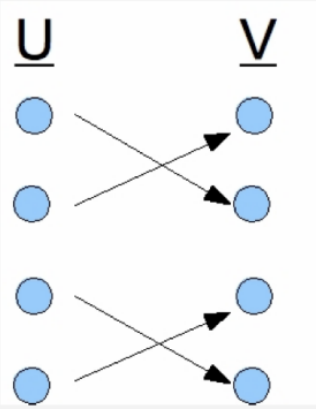
\includegraphics{images/image-1442319506.png}\\
The function is invertible because for every \(x, y \in U, f(x) = f(y)\)
and for every \(z \in V\), there exists \(x \in U\) such that
\(f(x) = z\).

\hypertarget{problem-0.8.7}{%
\subsubsection{Problem 0.8.7}\label{problem-0.8.7}}

Is the following function invertible? If yes, explain why. If not, can
you change the domain and/or codomain of the function to make it
invertible? Provide the drawing.\\
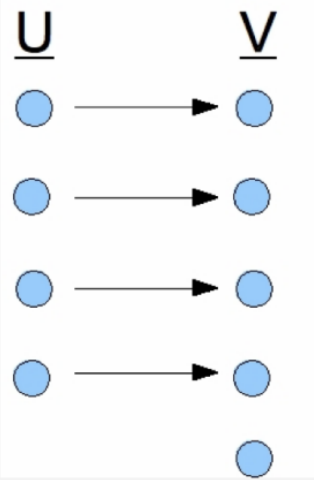
\includegraphics{images/image-1309870809.png}\\
The function is not invertible. It is impossible to make this function
invertible as it currently is now, as \(|V| \ne |U|\), but if you remove
the last element of \(V\), then it is invertible.

\hypertarget{problem-0.8.8}{%
\subsubsection{Problem 0.8.8}\label{problem-0.8.8}}

Let \(f : \mathbf{R} \rightarrow \mathbf{R}\) where \(f(x) = abs(x)\) .
Is there a choice of domain and codomain for the function \(g(x)\) with
the rule \(g(x) = \sqrt{x}\) such that \(g \circ f\) is defined? If so,
specify it. If not, explain why not. Could you change domain and/or
codomain of \(f\) or \(g\) so that \(g \circ f\) will be defined? The
choice of domain and codomain for \(g(x)\) where \(g \circ f\) is
defined is \(\mathbf{R}\).

\hypertarget{problem-0.8.9}{%
\subsubsection{Problem 0.8.9}\label{problem-0.8.9}}

Consider functions f and g in the following figure:

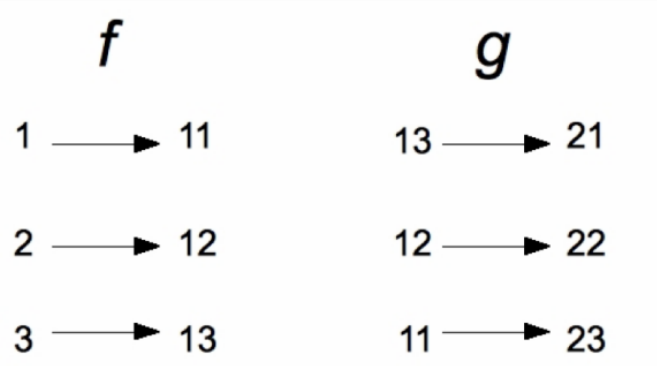
\includegraphics[width=3.70833in,height=\textheight]{images/image-1619342838.png}

Is \(f \circ g\) defined? If so, draw it, otherwise explain why not.

\(f \circ g\) is defined as follows:

\begin{figure}[H]

{\centering 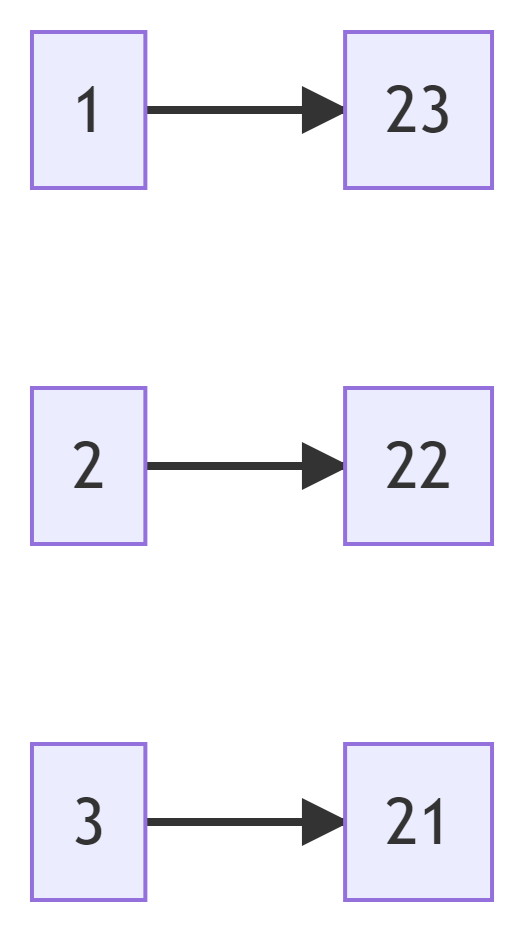
\includegraphics[width=1.6in,height=2.84in]{Chapter 0 Assignment_files/figure-latex/mermaid-figure-1.png}

}

\end{figure}

\hypertarget{problem-0.8.10}{%
\subsubsection{Problem 0.8.10}\label{problem-0.8.10}}

A function f(x) = x+1 with domain \{1, 2, 3, 5, 6\} and codomain \{2, 3,
4, 6, 7\} has the following probability on its domain: Pr(1) = 0.5,
Pr(2) = 0.2, and Pr(3) = Pr(5) = Pr(6) = 0.1. What is the probability of
getting an even number as an output of f(x)? An odd number?
\(\mathrm{Pr}("even") = \mathrm{Pr}(1) + \mathrm{Pr}(3) + \mathrm{Pr}(5) = 0.5+0.1+0.1 = 0.7\)

\hypertarget{problem-0.8.11}{%
\subsubsection{Problem 0.8.11}\label{problem-0.8.11}}

A function g(x) = x mod 3 with domain \{1, 2, 3, 4, 5, 6, 7\} and
codomain \{0, 1, 2\} has the following probability function on its
domain: Pr(1) = Pr(2) = Pr(3) = 0.2 and Pr(4) = Pr(5) = Pr(6) = Pr(7) =
0.1. What is the probability of getting 1 as an output of g(x)? What is
the probability of getting 0 or 2?
\(\mathrm{Pr}(\text{"1"}) = \mathrm{Pr}(1) + \mathrm{Pr}(4) + \mathrm{Pr}(7) = 0.2 + 0.1 + 0.1 = 0.4\)\\
\(\mathrm{Pr}(\text{"0 or 2"}) = \mathrm{Pr}(2) + \mathrm{Pr}(3)+\mathrm{Pr}+(5)+\mathrm{Pr}(6) = 0.2 + 0.2 + 0.1 + 0.1 = 0.6\)



\end{document}
